%!TEX root = ../../../super_main.tex

\section{ViewPagers} % (fold)
\label{sec:viewpagers}

% section viewpagers (end)

After the recent handover of GirafComponents from group \emph{SW604F15} to \emph{SW6013F15} it was discovered that a component in Pictosearch (developed by \emph{SW6013F15}) was not concistent with the design implemneted in the Launcher (implemented by \emph{SW604F15}) regarding showing of multiple items, apps and pictograms respectively. This inconsistency can be seen in \figref{fig:collab_with_group_13}, 

\begin{figure}[!htbp]
    \centering

    \begin{subfigure}[t]{0.4\textwidth}
        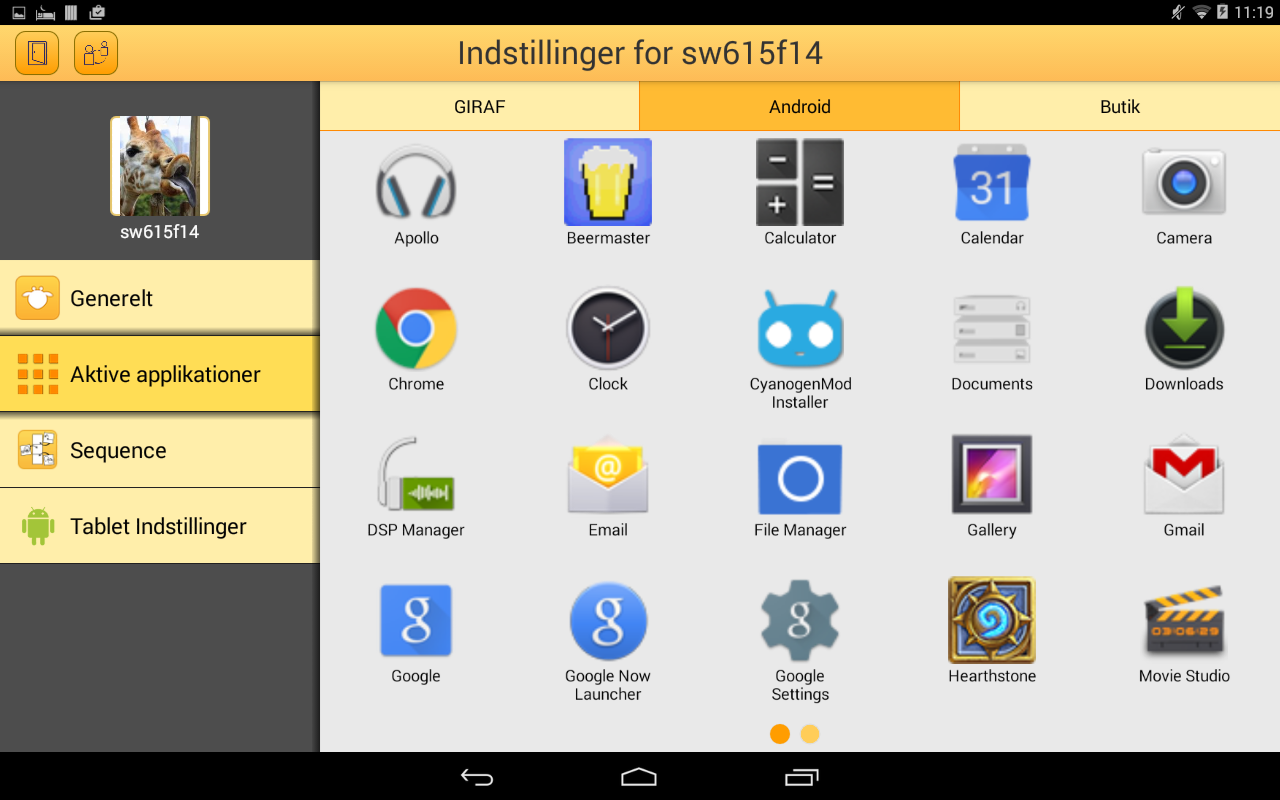
\includegraphics[width=\textwidth]{sprint_three/collab_with_group_13/launcher.png}
        \caption{\emph{GIRAF}-tab selected}
        \label{fig:collab_with_group_13_launhcer}
    \end{subfigure}
    \hspace{5em} 
    \begin{subfigure}[t]{0.4\textwidth}
        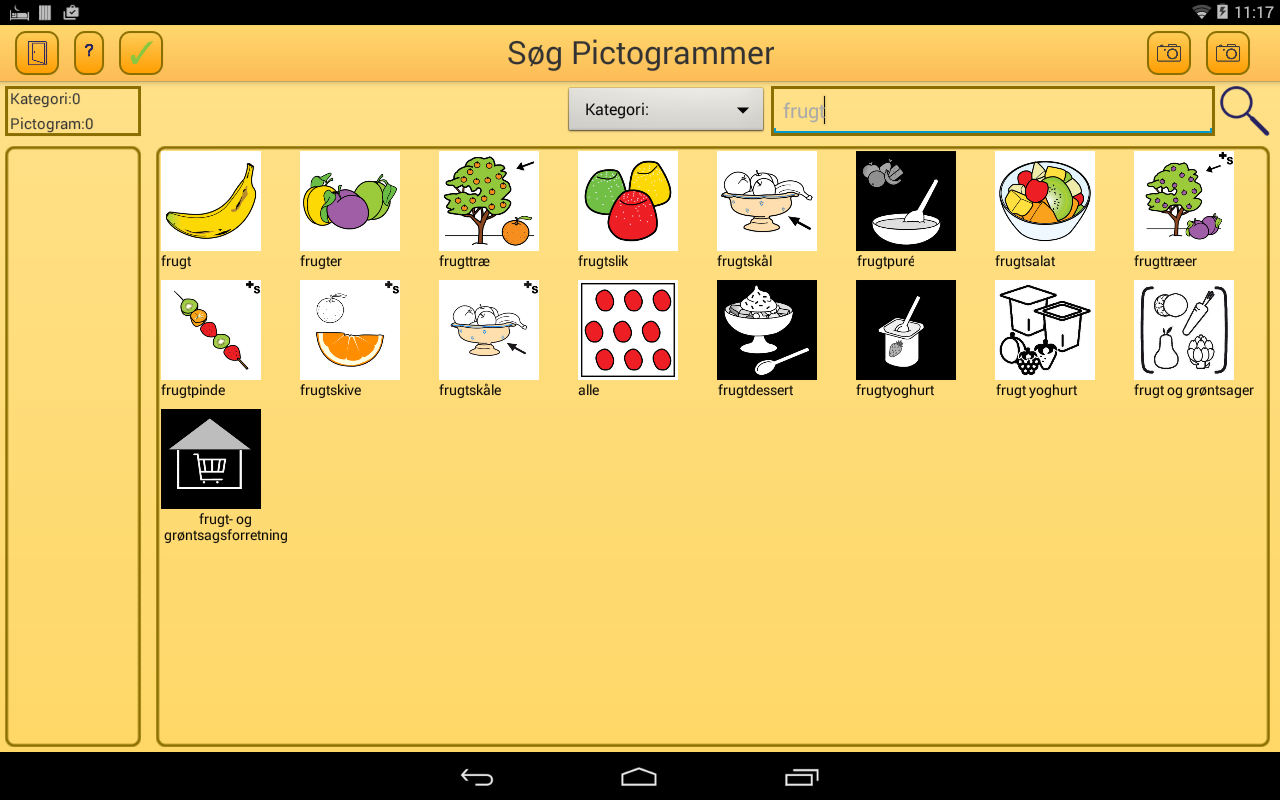
\includegraphics[width=\textwidth]{sprint_three/collab_with_group_13/pictosearch.png}
        \caption{\emph{Apps}-tab selected}
        \label{fig:collab_with_group_13_pictosearch}
    \end{subfigure}
    
    \caption{Problem visualized}
    \label{fig:collab_with_group_13}
\end{figure}

Since \emph{SW604F15} had already spent some time on implementing a viewpager for this purpose a soloution for Pictosearch was made in collaboration by these groups. A sligthly implementation difference was that the viewpager in the launcher is implementing a \androidinline{FragmentAdapter} where as the viewpager in Pictosearch is implemented using \androidinline{GridView}s. The final and update soloution can be sen on FIGREF.

\todo[inline]{Insert figure of final outcome of pictosearch}